% Licensed under the Creative Commons Attribution Share Alike 4.0 International.
% See the LICENSE file in the repository root for full license text.

\section{从官网上获取资源}

一般而言,前往官网下载软件资源是最好的选择。在搜索引擎搜索 CMake,发现其官网为 \url{https://cmake.org}。点击官网页面右上角的 Download 链接进入下载页面,在二进制分发文件(Binary distributions)中下载适合自己系统的 CMake。对于一般的 Windows 用户,下载 x64 安装包(Windows x64 Installer)即可。安装过程中需注意,请选择将 CMake 添加到系统 PATH 环境变量中,如图 \ref{fig:cmake-installment} 所示。

\begin{figure}[H]
	\centering
	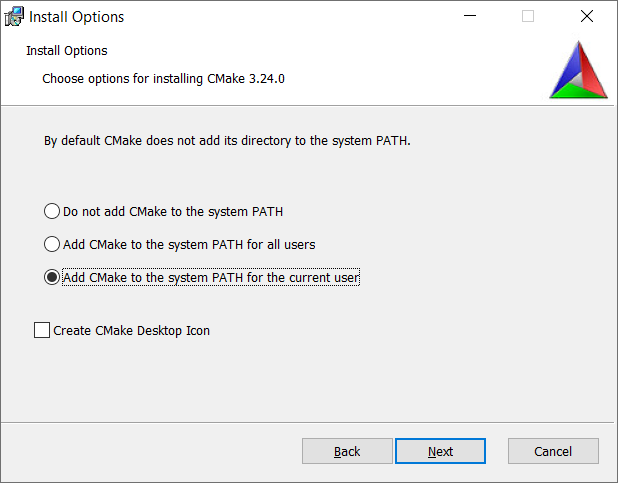
\includegraphics[width=0.6\linewidth]{assets/cmake-installment}
	\caption{安装 CMake 时,请选择添加 CMake 到系统 PATH 环境变量中。}
	\label{fig:cmake-installment}
\end{figure}

\begin{remark}
	现在,在最新的 Windows 操作系统中使用 \lstinline[language={}]{winget} 是更优的选择。
	打开终端,输入以下命令即可安装 CMake,省去了上网搜索的流程。

	\begin{lstlisting}[language={}, numbers=none]
winget install Kitware.CMake
	\end{lstlisting}

	其中包名 \lstinline[language={}]{Kitware.CMake} 可以使用 \lstinline[language={}]{winget find cmake} 命令找到。
\end{remark}

\bigskip

Linux 用户无需参考本文中关于软件安装与命令行使用的内容。但需要注意,不同 Linux 发行版附带的 CMake 版本不同,往往不是最新版本。

在官网页面右上角的链接中还能找到 CMake 的官方文档:\url{https://cmake.org/cmake/help/latest/}。它只能作为细则的参考,无法作为一份教程去学习——尽管其中附有一份教程\footnote{网址:\url{https://cmake.org/cmake/help/latest/guide/tutorial/index.html}。},但其质量不足以让你真正掌握 CMake,其中的部分内容也稍有过时。
